\documentclass[8pt,a5paper]{acm_proc_article-sp}
% fix umlauts
\usepackage[ngerman]{babel}
\usepackage[utf8]{inputenc} 
\usepackage[T1]{fontenc}  % Times new Roman
\usepackage{mathptmx}
\usepackage[]{blindtext}
\usepackage[a5paper, left=1.70cm, right=1.20cm, top=1.30cm, bottom=1.40cm]{geometry}
\usepackage{epstopdf}
% balance columns. original from acm doesn't work
\usepackage{balance}
% colors
\usepackage[compact]{titlesec}
\usepackage{natbib}
\titlespacing{\section}{0pt}{*0.7}{*0.5}

\usepackage[nolist]{acronym}
 
\usepackage[usenames,dvipsnames]{xcolor}
% automatic crosslinks
\usepackage[colorlinks=true,citecolor=black,linkcolor=black,filecolor=black,urlcolor=black,pagebackref=true]{hyperref}
\hypersetup{colorlinks=true,citecolor=black,linkcolor=black,filecolor=black,urlcolor=black,pagebackref=true}
%glossaries
%\usepackage{makeidx}
%\makeindex
%\usepackage[nomain]{glossaries}
%\makeglossaries
%\makeindex

\newcommand{\glspl}[1]{{#1}}

% http://en.wikibooks.org/wiki/LaTeX/Glossary
% http://mirror.informatik.uni-mannheim.de/pub/mirrors/tex-archive/macros/latex/contrib/glossaries/glossariesbegin.pdf

% Definitionsliste
\newcommand{\defitem}[1]{\item[#1]\phantomsection\label{#1}\hfill\\} 
\newcommand{\defref}[1]{\hyperref[#1]{#1}} 
\newcommand{\rem}[1]{}
% Marking colors
\definecolor{todo}{rgb}{1,0.2,0.2}
\definecolor{reconsider}{rgb}{0.6,0.6,0.3}
\newcommand{\todo}[1]{{\color{todo} #1}}
\newcommand{\reconsider}[1]{{\color{reconsider} #1}}



\graphicspath{{img/}{./}}
\usepackage{graphicx}
\title{Portable System to Detect driver drowsiness with Body Sensors (PoSDBoS) \titlenote{ \scriptsize 
  \flushleft Betreuer Hochschule:  \ \ Prof. Dr. Martinez\\ 
  \qquad \qquad \qquad \qquad \quad \ \  Hochschule Reutlingen\\ 
  \qquad \quad \quad \quad \qquad \qquad \ \ Natividad.Martinez@Reutlingen-\\
  \qquad \qquad \qquad \qquad \quad \ \ University.de \\
  \includegraphics[width=1.8cm]{iot_hs_rt} \ \ \quad Master Project IoT 2016\\
  \ \ \\
  31. Juli 2016, Hochschule Reutlingen\\ 
  \copyright  ~ 2016 Paul Pasler}}


\numberofauthors{3}
\author{
	\alignauthor
	  \center
		\aufnt{Paul Pasler}\\
          \affaddr{Reutlingen University}\\
        \textbf{\textsf{Paul.Pasler@Student.Reutlingen-University.DE}}
}


\begin{document}
\begin{acronym}
\acro{FAS}{Fahrerassistenzsystem}
\acro{FASs}{Fahrerassistenzsysteme}
\acro{ME}{Müdigkeitserkennung}
\acro{MESs}{Müdigkeitserkennungssysteme}
\acro{ADAS}{Advanced Driver Assistance System}
\acro{ADASs}{Advanced Driver Assistance Systems}
\acro{bspw}{beispielsweise}
\acro{RTU}{Reutlingen University}
\acro{BS}{Körpersensoren}
\end{acronym}


\maketitle
\sloppypar{
\begin{abstract}
\acl{FASs} sind aus modernen Fahrzeugen nicht mehr wegzudenken. \acl{ME} hilft Sekundenschlaf oder müdigkeitsbedingte Unachtsamkeit zu vermeiden und verhindert somit schwere Unfälle. Systeme mit Body-Sensorik zeigen in verschiedenen Studien sehr genau Ergebnisse und erkennen Müdigkeit frühzeitiger als andere Ansätze. In der vorgelegten Arbeit wurde ein solches System mit einem Elektroenzephalogramm (EEG) umgesetzt und getestet. Hierfür wurden Testdaten aufgenommen, verarbeitet und klassifiziert, sodass der aktuelle Status des Fahrers "`Wach"' oder "`Müde"' erkannt werden kann.

\end{abstract}

\keywords{
\acl{FAS}, \acl{ME}, Elektroenzephalogramm, Signalverarbeitung, Machine Learning
}

\category{A.0}{ACM}{
Experimentation
}


\section{Einleitung}
\label{chap:intro}
Fristeten \acl{FASs} vor wenigen Jahren ein Nischendasein in Oberklassewagen, werden sie immer günstiger und beliebter. Mittlerweile halten sie auch in Mittelklasse- und Kleinwagen Einzug. Die Unternehmensberatung Strategy Analytics geht in den nächsten Jahren von einer Versechsfachung von verbauten \acl{FASs} aus \cite{strategy_analytics}. Denn sie erhöhen den Komfort und helfen bei der Vermeidung schwerer Unfälle. So schätzt die Boston Consulting Group, dass durch den flächendeckenden Einsatz von \acl{FASs}, die Unfallrate in den USA um bis zu 28\% zurückgehen könnte \cite{bcgperspectives}. \acl{ME} ist eines dieser Systeme zur Vermeidung von müdigkeitsbedingter Unachtsamkeit oder Sekundenschlaf. Beispielsweise rät die \acl{ME} "`Attention Assist"' von Daimler dem Fahrer, zu gegebenen Anlass, eine Pause einzulegen und zeigt ein Kaffeesymbol im Cockpit an \cite{Daimler}. Denn laut dem Deutschen Verkehrssicherheitsrat zählt Müdigkeit, neben überhöhter Geschwindigkeit, zu den häufigsten Unfallursachen und ist damit für jeden fünften schweren Unfall verantwortlich \cite{dvr_statistic}. In einer Studie der amerikanischen "`National Sleep Foundation"' \cite{nsf_statistic}, gab die Hälfte der Befragten an, dass sie schon einmal schläfrig gefahren seien und fast jeder dritte sogar kurz am Lenkrad eingeschlafen war. Dies zeigt die Wichtigkeit einer Erkennung von Müdigkeit und einer Meldung an den Fahrer.


\begin{figure*} 
  \begin{center}
    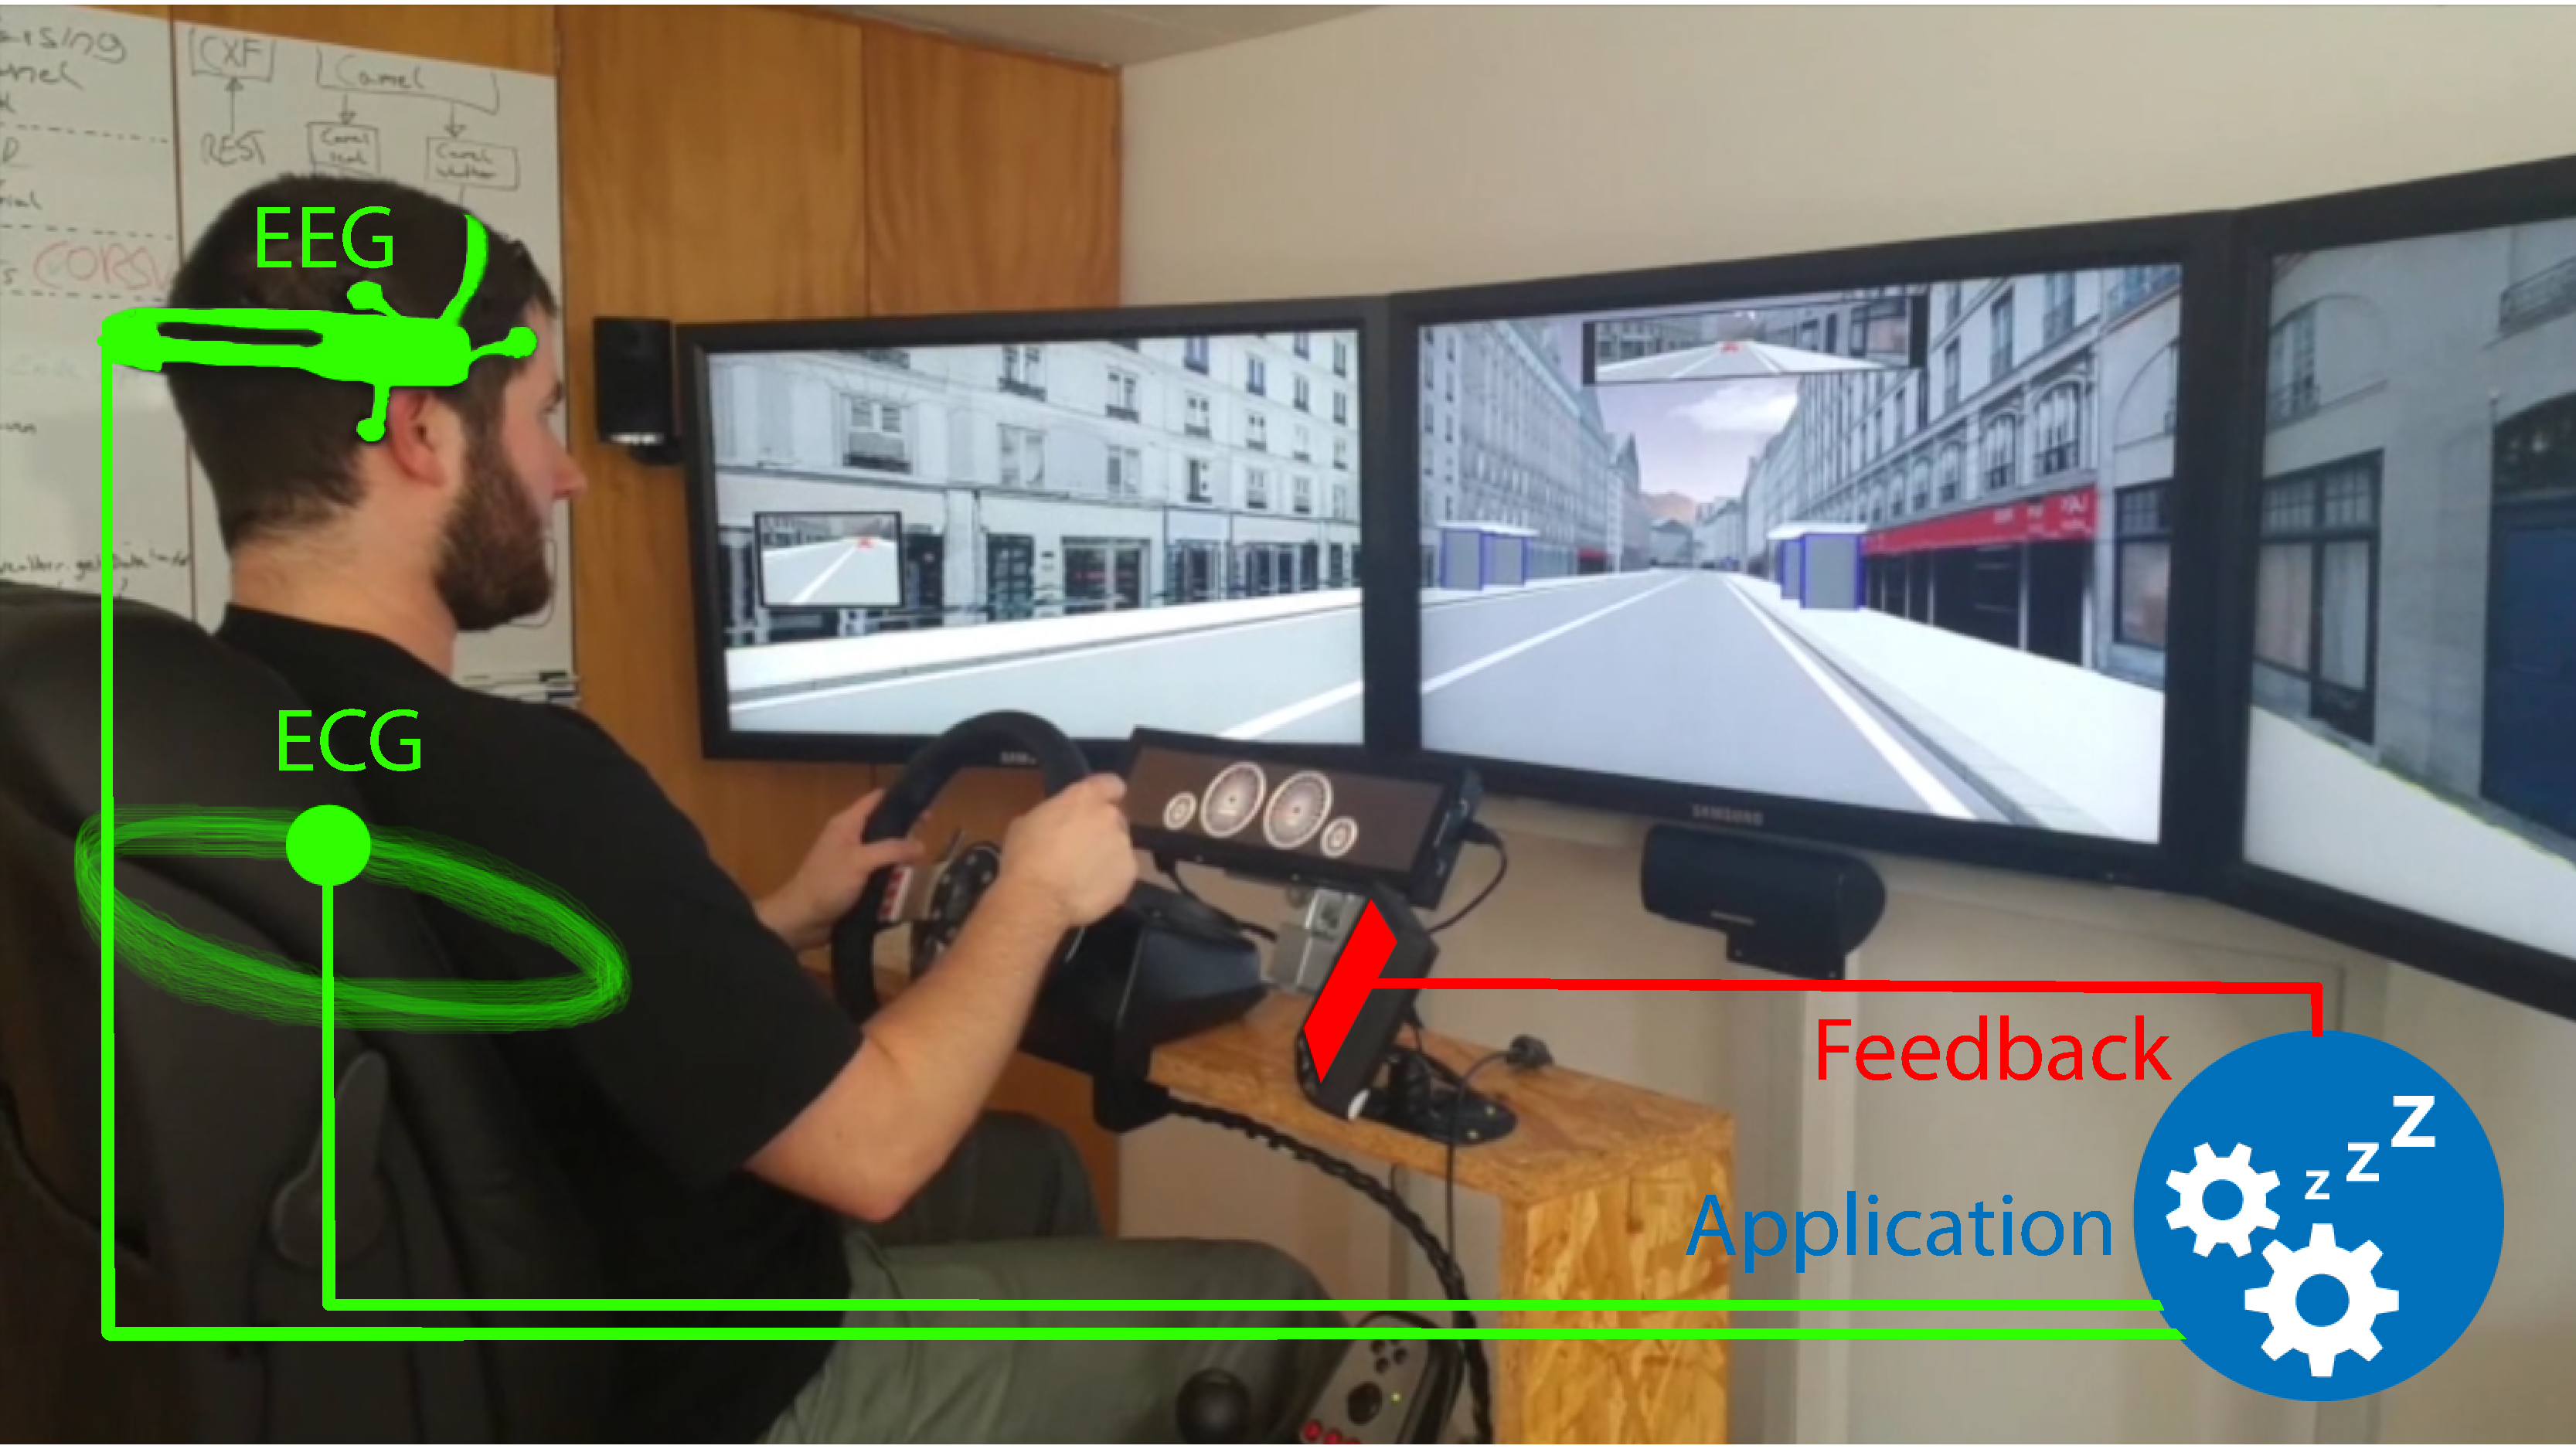
\includegraphics[width=12cm]{aufbau}
    \caption{Skizze des Systemaufbaus: \acl{BS} (Elektroenzephalografie / Elektrokardiogramm) liefert Daten an die Applikation und ein Feedback-Device warnt den müden Fahrer. Bild zeigt den Fahrsimulator der \acl{RTU}.}
    \label{fig:sketch}
  \end{center}
\end{figure*}

Um das Risiko eines Unfalls auf Grund von Übermüdung zu senken, soll langfristig ein multimodales System zu \acl{ME} entwickelt werden (Siehe Abb. \ref{fig:sketch}). Solche Systeme existieren bereits, es fehlt jedoch oftmals an Komfort und Portabilität. Ziel dieser Arbeit ist es, aktuelle Arbeiten zu diesem Thema zu sichten und ein Konzept für ein solches System mit \acl{BS} zu erstellen. Die \acl{BS} messen Signale direkt am Körper und können somit sofort auf Veränderungen reagieren. Ein Algorithmus versucht an Hand der Messdaten zu erkennen, ob der Fahrer übermüdet. Diese Systeme müssen richtig und genau funktionieren, sodass die Sicherheit zu jeder Zeit gewährleistet ist. Da die Sensoren direkt am Körper anliegen, können sie den Fahrer beeinträchtigen. Das Problem der invasiven Sensoren soll weitestgehend eliminiert und den Fahrer wenig bis gar nicht stören. Feldversuche eignen sich nicht zur Entwicklung eines solchen Systems, da Eigen- und Fremdgefährdung eines übermüdeten Fahrers nicht vertretbar sind. Das System soll darum im Simulationsumfeld der \acl{RTU} entwickelt und getestet werden. Dennoch müssen die Ergebnisse einem Test im Straßenverkehr standhalten, da es unter Umständen zu anderen Signalen, \acl{bspw} aufgrund von erhöhtem Stress, kommen kann. Darum soll das System später leicht in ein echtes Fahrzeug portiert und validiert werden können. Gelingt dies, kann es zudem mit anderen Systemen gekoppelt zu werden, um das Ergebnis insgesamt zu verbessern. Damit hilft das vorgestellte Konzept, den Fahrer vor einer drohenden Müdigkeit zu warnen und so schwere Unfälle zu vermeiden.\\ 

Die Ausarbeitung gliedert sich folgendermaßen. Im Kapitel \ref{chap:me} werden verschiedene Forschungsergebnisse zur \acl{ME} aufgezeigt und in Kapitel \ref{chap:an} verglichen. Das Konzept eines portablen Systems zur \acl{ME} mit \acl{BS} wird im Kapitel \ref{chap:prop} vorgestellt. Der Versuchsaufbau und das Testszenario im Simulationsumfeld der \acl{RTU} ist Thema von Kapitel \ref{chap:eval}. Das Ergebnis und weitere Schritte werden in Kapitel \ref{chap:outro} beschrieben. In den anschließenden Absätzen werden Grundlagen für die kommenden Kapitel erläutert.


\balance
\bibliographystyle{unsrt} % abbrv, alpha, plain, unsrt, apalike
\bibliography{Quellen}


\end{document}
